\documentclass{article}

% if you need to pass options to natbib, use, e.g.:
   %  \PassOptionsToPackage{numbers, compress}{natbib}
%before loading neurips_2019 



% ready for submission
% \usepackage{neurips_2019}

% to compile a preprint version, e.g., for submission to arXiv, add add the
% [preprint] option:
%     \usepackage[preprint]{neurips_2019}

% to compile a camera-ready version, add the [final] option, e.g.:
    \usepackage[final]{neurips_2019}
\bibliographystyle{unsrtnat}

% to avoid loading the natbib package, add option nonatbib:
   %\usepackage[nonatbib]{neurips_2019}

\usepackage[utf8]{inputenc} % allow utf-8 input
\usepackage[T1]{fontenc}    % use 8-bit T1 fonts
\usepackage{hyperref}       % hyperlinks
\usepackage{url}            % simple URL typesetting
\usepackage{booktabs}       % professional-quality tables
\usepackage{amsfonts}       % blackboard math symbols
\usepackage{nicefrac}       % compact symbols for 1/2, etc.
\usepackage{microtype}      % microtypography
\usepackage{hyperref}
\usepackage{graphicx}
\usepackage{subcaption}
\usepackage{geometry}
\usepackage{float}
\graphicspath{{./images/}}
\title{Project Report-Deep Learning (COMP 5970/6970) }



% The \author macro works with any number of authors. There are two commands
% used to separate the names and addresses of multiple authors: \And and \AND.
%
% Using \And between authors leaves it to LaTeX to determine where to break the 

% lines. Using \AND forces a line break at that point. So, if LaTeX puts 3 of 4
% authors names on the first line, and the last on the second line, try using
% \AND instead of \And before the third author name.

\author  {%
  Charles Tripp Isbell \\
  Auburn University\\
  \texttt{cai0004@auburn.edu}\\
  \And
  Lalithya Kuntamukkala\\
  Auburn University\\
  \texttt{lzk0034@auburn.edu}\\
  \And
  James Lee\\
  Auburn University\\
  \texttt{jyl0003@auburn.edu}\\}
  
 
\newcommand{\subf}[2]{%
    {\small\begin{tabular}[t]{@{}c@{}}
    #1\\#2
    \end{tabular}}
}

\begin{document}


\maketitle{}

\begin{abstract}
  We use the Network Dissection / GAN Dissection to analyze and reason about a few generative models: pix2pix, and StyleGAN. We dissect a Progressive GAN to get us started and to use as a comparative baseline to reason about the other two. We train and dissect a pix2pix model in the hopes that it would have uniquely high levels of interpretability, and our hopes mostly fall short. We dissect a StyleGAN model to interesting and surprising results.
\end{abstract}

\section{Introduction}
\label{gen_inst}

In the recent years, there has been a slew of research in the field of Deep Learning has worked towards the goal of visualizing and understanding deep neural network architectures.  Supervised learning with convolutional networks (CNNs) has been probed to a much deeper extent when compared with unsupervised learning using CNNs in computer vision applications. Visualizing intermediate layer activations, visualizing convnet filters, class activation map (CAM) visualizations (\cite{classactmap}) are some of the techniques used in visualizing CNNs. In CAM visualization, a heat map of class activations is produced, which indicates how important a location for a given output class. Network Dissection is a general framework, belonging to the class of CAM visualizations, for quantifying the interpretability of latent representations of CNNs by evaluating the alignment between individual hidden units and a set of semantic concepts (\cite{netdissect}). 

Generative models are a fundamental component of a variety of important machine learning and computer vision algorithms. The field of generative models is booming, and from it many unique models have emerged including GANs and VAEs. A dominant/popular model for image generation is the Generative Adversarial Network(\cite{gan}). The GAN model architecture involves two sub-models: a generator model for generating new examples and a discriminator model for classifying whether generated examples are real, from the domain, or fake, generated by the generator model. The two models, the generator and discriminator, are trained together. The generator generates a batch of samples, and these, along with real examples from the domain, are provided to the discriminator and classified as real or fake. The discriminator is then updated to get better at discriminating real and fake samples in the next round, and importantly, the generator is updated based on how well, or not, the generated samples fooled the discriminator.  

This exploration has given way to new research into understanding generative models. Bau et al. [2019] adapt their method from Bau et al. [2017] and build on it to understand and reason about GANs. 

\section{Related Works}

\subsection{GAN Dissection}
This paper (\cite{gandissect}) presents a framework to visualize and understand GANs at the unit-, object-, and scene-level. It aims to understand how different objects and classes of objects are encoded by the GAN. A group of interpretable units that are closely related to object concepts are identified using a segmentation-based network dissection method. The causal effect of interpretable units is quantified by measuring the ability of interventions to control objects in the output. The contextual relationship between these units and their surroundings is examined by inserting the discovered object concepts into new images. 

Many parts of GAN representations can be interpreted, not only as signals that correlate with object concepts but as variables that have a causal effect on the synthesis of objects in the output. These interpretable effects can be used to compare, debug, modify and reason about a GAN model. In the paper, \cite{gandissect} dissect a Progressive GAN from \cite{progan}. They released a tool along with their paper on \texttt{https://github.com/CSAILVision/GANDissect} for general purpose GAN dissection which we seek to use to study other models.

\subsection{StyleGAN}
 StyleGAN \cite{stylegan} allows for more control in the image synthetic process. This is possible in the ways that the StyleGAN generator was redesigned. Using a mapping network of eight fully connected layers and getting a learned constant, this allows the model to generate a vector that can reduce the correlation between features. Then, learned affine transformations then embed the vector to styles that then control the adaptive instance normalization(AdaIn) where each feature map is normalized separately, and then scaled and biased using scalar components from the style. Lastly, "explicit noise inputs" are then introduced to generate stochastic detail. Compelling enough, this design led to improved generated image quality. Combined with that the generator architecture makes it possible to control the image synthesis through scale-specific modifications to the styles, we believe that this GAN model is a good candidate for our project because it is an interesting alternative extension to ProGan and that we can utilize tools that the Gan Dissection paper used as well. Lastly, we believe that studying and performing GAN dissection on this model could lead to interesting results.

\subsection{Pix2pix}
Most studies in the field of GANs have been focused on image synthesis from a random vector z. Conditional GANs are improved and used as a general-purpose solution to image-to-image translation problems. It can also be used for colorization and super-resolution of input images. The conditioning image, x is applied as the input to the generator and to the discriminator. The loss function is a Dual Objective Function with Adversarial and L1 Loss. Image Synthesis architectures typically take in a random vector of size 100x1, project it into a higher dimensional vector with a fully connected layer, reshape it, and then apply a series of de-convolutional operations until the desired spatial resolution is achieved. In contrast, the Generator in pix2pix resembles an auto-encoder. The generator compresses the input image and then learns how to upsample it to the output image. Because of this unique structure we think it would be interesting to observe through the dissection framework.

\section{Methods}
Our methods for this project involve researching other GAN models we think might yield interested results when studied under the GAN Dissection Bau et al. [2019] framework. A pre-trained GAN and a segmented dataset are to be examined. The GAN dissection tool released by Bau et al. [2019] at http://github.com/CSAILVision/GANDissect is applied, which carries out dissection on the specified model, and this basically carries out the heavy lifting. The tool also produces metrics and visualizations of sets of units with high agreement with specified concepts which we can then use in our analysis.

A Google Compute Engine with a single T4 (the tool only uses one GPU) is used for all dissections and training. All of the dissections are carried out using the tool provided by \cite{gandissect} \texttt{https://github.com/CSAILVision/GANDissect} released along with the paper. This tool is set up to hook into a PyTorch model to retain its layer activations and perform interventions, so we converted the official TensorFlow implementation of StyleGAN to Pytorch to be compatible. Since different datasets could have significant effects on the object representations in a network, we wanted to stick with the various LSUN datasets (\cite{lsun}) used in the original paper so that our results would remain comparable. 

\subsection{Progressive GAN}
First we replicate one of the dissections in \cite{gandissect} by dissecting one of the Progressive GANs (\cite{progan}) provided with the paper that is pre-trained on the LSUN living room dataset (256x256). We use this as a baseline to check that our results match along with theirs, and to have something to compare to when doing interventions on the other models. Since we only measure Intersection Over Union for this project and not average causal effect, we don't have a way to quantitatively compare the causality of units or how "easily" manipulable a generator's output is through interventions. So having the baseline to compare interventions on other models with gives us some sort of sense of this, even though it's not exactly measurable. 

\subsection{Pix2pix}
Next we try dissection on a Pix2Pix generator (\cite{pix2pix}). Since there were no pre-trained pix2pix models on LSUN or anything similar (the closest we could find was the facades model, but that seemed to lack the diversity in object classes for our purposes) we first train our own pix2pix model. To do this, we first segment the LSUN church outdoor 256x256 dataset using a Unified Perceptual Parser (\cite{segmenter}) to produce semantic segmentations for each church image. We then use these segmentation / image pairs to train a pix2pix Unet-256 model from \href{https://github.com/junyanz/pytorch-CycleGAN-and-pix2pix}{pytorch-CycleGAN-and-pix2pix} (\cite{pix2pix}) to train a PyTorch model compatible with the dissection tool. We trained this for two days, and the results were... not stellar, so this may either have been due to (somewhat) messy segmentations or just not enough training time. Then we modified the dissection tool to generate outputs using some of the church segmentations we sat aside from training the model. And then the outputs during the dissection process are of course re-segmented again for the IoU measurements, leading to a somewhat circular process of ending up where we started (it would be interesting to instead run the classifier case (Network Dissection \cite{netdissect}) on the segmented inputs, though perhaps not that interesting).

\subsection{StyleGAN}
Finally, we also ran dissection on StyleGAN for some pretty interesting results. We converted the official TensorFlow implementation from \cite{stylegan} to PyTorch to be compatible with the network dissection tool and used the pre-trained LSUN bedrooms 256x256 model provided by \cite{stylegan}.
\section{Experiments and Results}
\begin{figure}[h!]
\caption{Progressive GAN layers: Interpretable units distribution and highest IoU unit sample images}
\begin{tabular}{c c }
    \begin{subfigure}[h!]{0.6\textwidth}
        \caption{Layer 1 interpretable units (2/512)}
        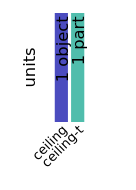
\includegraphics[scale=0.33]{pg_layer1.png}
    \end{subfigure} &
    \begin{subfigure}[h!]{0.4\textwidth}
        \caption{Unit 457: ceiling with 0.12 IoU}
        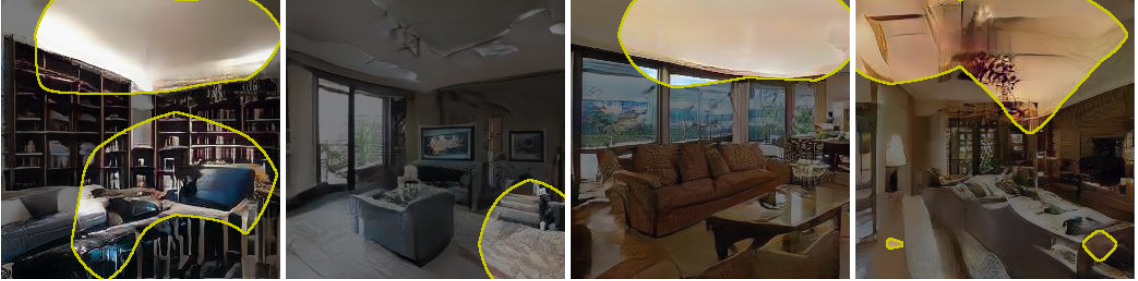
\includegraphics[scale=0.16]{pg_layer1_u457_ceil_0.12.png}
    \end{subfigure} \\
    \begin{subfigure}[h!]{0.6\textwidth}
        \caption{Layer 4 interpretable units (241/512)}
        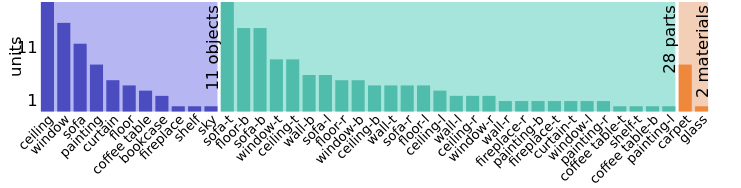
\includegraphics[scale=0.33]{pg_layer4.png}
    \end{subfigure} &
    \begin{subfigure}[h!]{0.4\textwidth}
        \caption{Unit 306: ceiling 0.32 IoU}
        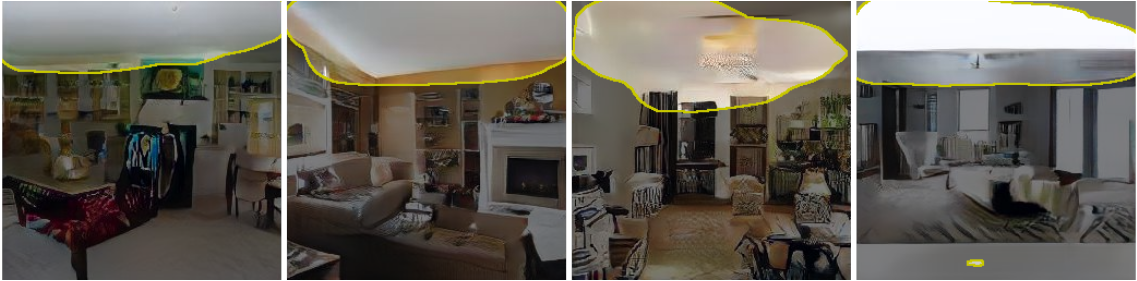
\includegraphics[scale=0.16]{images/pg_layer4_unit306_ceil_0.32.png}
    \end{subfigure} \\
    \begin{subfigure}[h!]{0.6\textwidth}
        \caption{Layer 7 interpretable units (122/256)}
        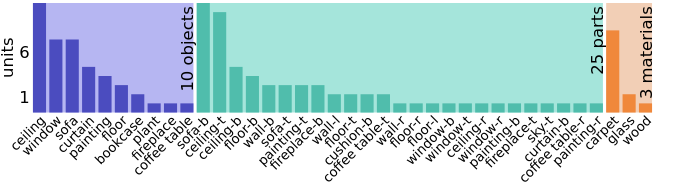
\includegraphics[scale=0.33]{pg_layer11.png}
    \end{subfigure} &
    \begin{subfigure}[h!]{0.4\textwidth}
        \caption{Unit 172: ceiling 0.34 IoU}
        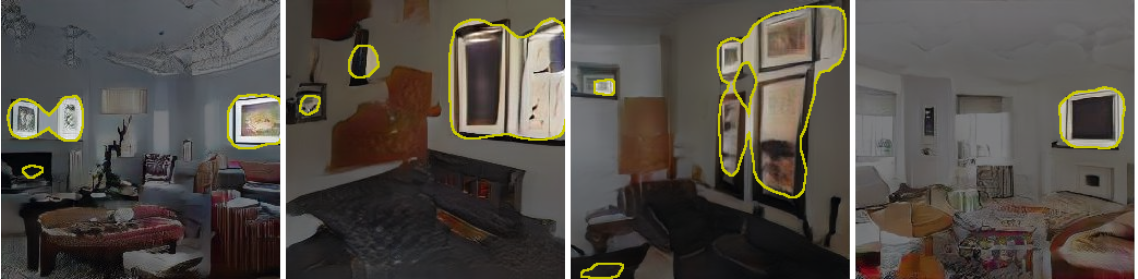
\includegraphics[scale=0.16]{images/pg_layer7_u172_ceil_0.34.png}
    \end{subfigure} \\
\end{tabular}
\end{figure}
\subsection{Progressive GAN}
We (perhaps unsurprisingly) found very similar results to those in \cite{gandissect} in our replication. The "interpretable" units distributions in our results for layers 1, 4, and 7 are extremely similar to theirs, so with that we conclude that these results present a reliable baseline for us to compare against. (This isn't super important to have since we're not really making quantitative claims or anything, we just wanted to make sure that we could get the tool working)

\subsection{Pix2Pix}
With pix2pix, the idea we had was that they segmented inputs would result in a more disentangled object representation, and maybe we'd be able to use that and alter the output image significantly by intervening within the network. This would perhaps indicate the possibility of optimizing the latent space to lead to more disentangled (and thus more controllable) networks. However, what we found didn't quite seem to be the case, and its unclear if that's because of something specific to pix2pix, or if we didn't train the model long enough or the segmentation we trained off of weren't great. The results we got after training for two day's weren't great.

\begin{figure}[h!]
    \caption{Segmentations and generated/real images from our pix2pix}
    \centering
    \begin{subfigure}[h!]{0.3\textwidth}
        \caption{input seg}
        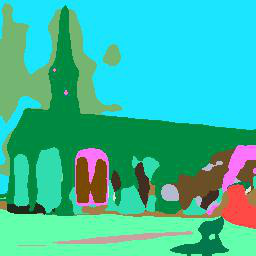
\includegraphics[scale=0.3]{110008_real_A.png}
    \end{subfigure}
     \begin{subfigure}[h!]{0.3\textwidth}
        \caption{output}
        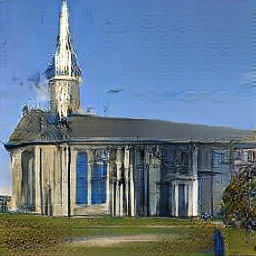
\includegraphics[scale=0.3]{110008_fake_B.png}
    \end{subfigure}
     \begin{subfigure}[h!]{0.3\textwidth}
        \caption{real (or is it?) (it is)}
        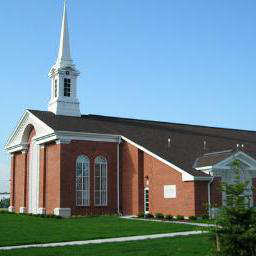
\includegraphics[scale=0.3]{110008_real_B.png}
    \end{subfigure}\\
     \begin{subfigure}[h!]{0.3\textwidth}
        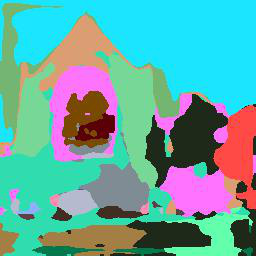
\includegraphics[scale=0.3]{110013_real_A.png}
    \end{subfigure}
     \begin{subfigure}[h!]{0.3\textwidth}
        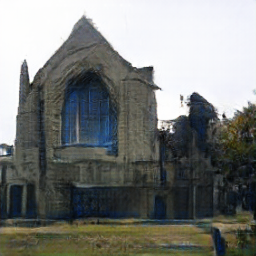
\includegraphics[scale=0.3]{110013_fake_B.png}
    \end{subfigure}
     \begin{subfigure}[h!]{0.3\textwidth}
        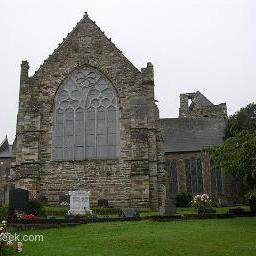
\includegraphics[scale=0.3]{110013_real_B.png}
    \end{subfigure}
\end{figure}

Looking at how long it took them to train StyleGAN (though that's certainly a more complicated task than pix2pix), it seems like we probabily just didn't train it for long enough. However our segmentations are kind of messy, unlike the ones that they use in the  labels2images examples with the paper (\cite{pix2pix}), so that could certainly be an issue as well. 

Our results from the dissection did not indicate the interpretability we were hoping for, and that's possibly due to the poor quality of the output images (of which many had significant artifacting). We chose to dissect layers 5, 9, and 12, since layer 9 is the middle of the Unet "bottleneck" and we were wondering what was going on in there (it turns out, not much that we could understand) and layers 5 and 12 are sort of opposite each other in the downsampling / upsampling sequence and we wondered if they might share some similarities due to skip-connections and such. 


So there weren't many intepretable units for each layer: 158/512 with IoU $\geq$ 0.05 for layer 5, 119/512 for layer 9, and 90/512 for layer 12. This seemed to be reflected in how much we could affect the output using insertions/ablations as well. One thing we did notice when messing around with interventions was that the output image would adhere to the "outline" of the segmentation it was translated from. We could adjust textures of the shapes, but the shapes themselves were very much set in stone by the segmentation, so our hopes of being able to paint an output image from the inside of the network similar to how you could paint it at the segmentation input were dashed. That being said, the low interpretability could certainly be a result of our low quality generated images, and we still think it would be an interesting idea to follow through with a proper generator. 

Also, that portal to the underworld artifact on many of those images seemed to appear after the first day of training. While we don't know what caused it or what it is, we were able to identify and ablate some of the units responsible.

\begin{figure}[h!]
    \centering
    \caption{artifacted images on top, corrected units on bottom}
    \begin{tabular}{c  c c  c }
    \begin{subfigure}[h!]{0.25\textwidth}
        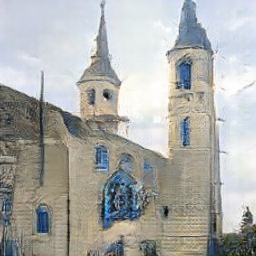
\includegraphics[scale=0.3]{images/25artifact.jpg}
        \\
        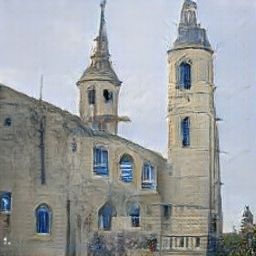
\includegraphics[scale=0.3]{images/25noartifact.jpeg}
    \end{subfigure} &
    \begin{subfigure}[h!]{0.25\textwidth}
       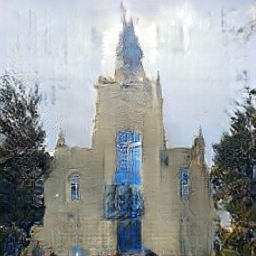
\includegraphics[scale=0.3]{images/37artifact.jpg}
    \\
        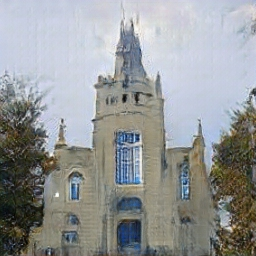
\includegraphics[scale=0.3]{images/37noartifact.jpeg}
    \end{subfigure} &
     \begin{subfigure}[h!]{0.25\textwidth}
        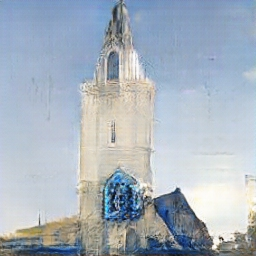
\includegraphics[scale=0.3]{images/43artifact.jpg}
        \\
        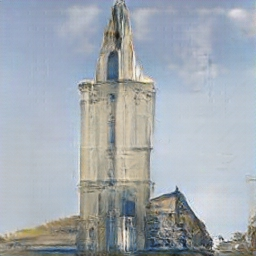
\includegraphics[scale=0.3]{images/43noartifact.jpeg}
    \end{subfigure} &
    \begin{subfigure}[h!]{0.25\textwidth}
        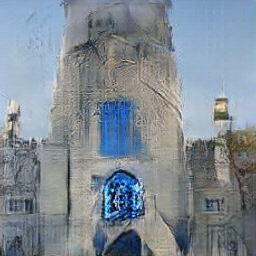
\includegraphics[scale=0.3]{images/77artifact.jpg}
        \\
        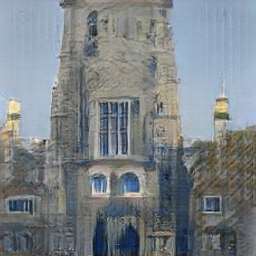
\includegraphics[scale=0.3]{images/77noartifact.jpeg}
    \end{subfigure}
    \end{tabular}
\end{figure}

\begin{figure}[h!]
\caption{Pix2Pix layers: Interpretable units distribution and highest IoU unit sample images}
\begin{tabular}{c c }
    \begin{subfigure}[h!]{0.3\textwidth}
        \caption{Layer 5 interpretable units (158/512)}
        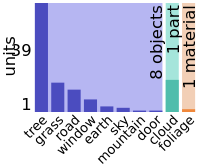
\includegraphics[scale=0.5]{p2p_layer5.png}
    \end{subfigure} &
    \begin{subfigure}[h!]{0.5\textwidth}
        \caption{Unit 164: sky with 0.65 IoU}
        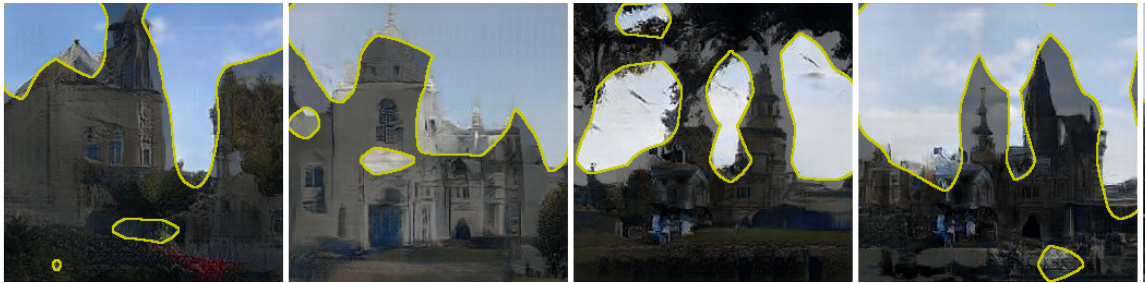
\includegraphics[scale=0.25]{images/p2p_layer5_unit164_0.65iou.png}
    \end{subfigure} \\
    \begin{subfigure}[h!]{0.3\textwidth}
        \caption{Layer 9 interpretable units (119/512)}
        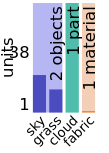
\includegraphics[scale=0.5]{images/p2p_layer9.png}
    \end{subfigure} &
    \begin{subfigure}[h!]{0.5\textwidth}
        \caption{Unit 458: sky 0.58 IoU}
        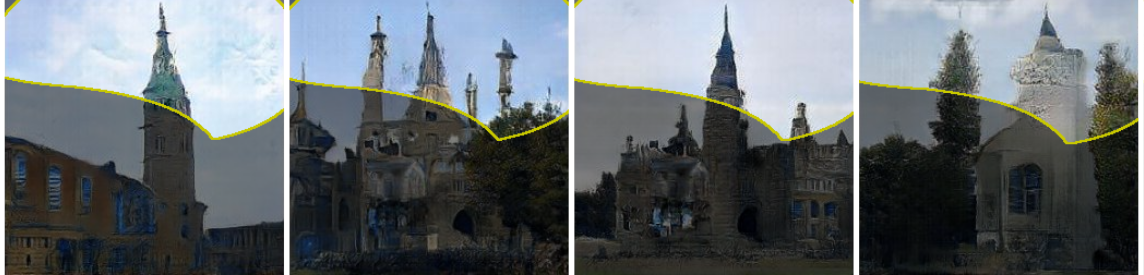
\includegraphics[scale=0.25]{images/p2p_layer9_unit458_0.58iou.png}
    \end{subfigure} \\
    \begin{subfigure}[h!]{0.3\textwidth}
        \caption{Layer 12 interpretable units (90/512)}
        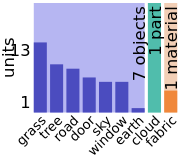
\includegraphics[scale=0.5]{images/p2p_layer12.png}\hspace{2em}
    \end{subfigure} &
    \begin{subfigure}[h!]{0.5\textwidth}
        \caption{Unit 270: sky 0.59 IoU}
        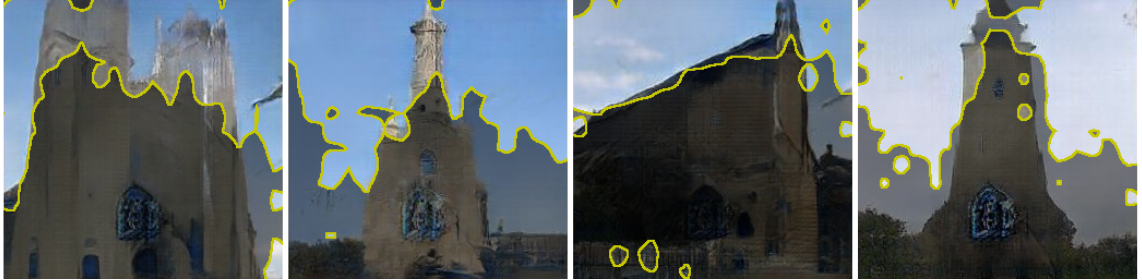
\includegraphics[scale=0.25]{images/p2p_layer12_unit270_iou0.59.png}
    \end{subfigure} \\
\end{tabular}
\end{figure}

\newpage
\subsection{StyleGAN}
StyleGAN, on the other hand, yielded some pretty interesting (and surprising) results. StyleGAN touts a highly disentangled network through its intermediate latent space. While they're talking about latent space disentanglement, we think that this might also be reflected by increased interpretable representations within the network (it sort of, at least to our intuition, aligns with the idea of linear separability that they speak of in \cite{stylegan}). The results seem to reflect that as well, as after running dissection on the pretrained LSUN bedrooms styleGAN, we found that it contained a surprising "amount" of interpretability. That is, not only did it contain a large number of interpretable units (units with IoU $\geq$ 0.05 for some class), but the IoU of many of the units was extraordinarily high compared to the Progressive GAN we originally dissected. Even more surprising to us, however, was that we thought that this might also indicate a greater causality of those units, in that we would have more control over the output through interventions. This proved not to be the case however, as no matter how hard we hacked away at more and more units, we could rarely erase any units from the output image. 


\begin{figure}[h!]
\caption{StyleGAN layers: Interpretable units distribution and highest IoU unit sample images}
\hspace{-3em}\begin{tabular}{c c }
    \begin{subfigure}[h!]{0.6\textwidth}
        \caption{Layer 3 interpretable units (258/512)}
        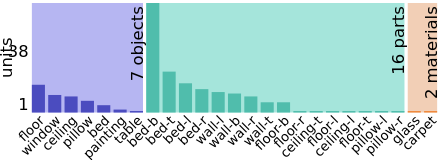
\includegraphics[scale=0.4]{images/sg_layer3.png}
    \end{subfigure} &
    \begin{subfigure}[h!]{0.5\textwidth}
        \caption{Unit 52 bed 0.48 IoU}
        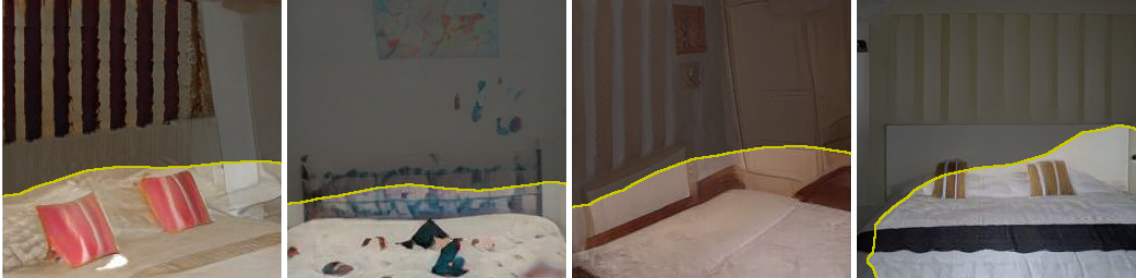
\includegraphics[scale=0.2]{images/sg_layer3_unit52_bedIoU_0.48.png}
    \end{subfigure} \\
    \begin{subfigure}[h!]{0.6\textwidth}
        \caption{Layer 6 interpretable units (387/512)}
        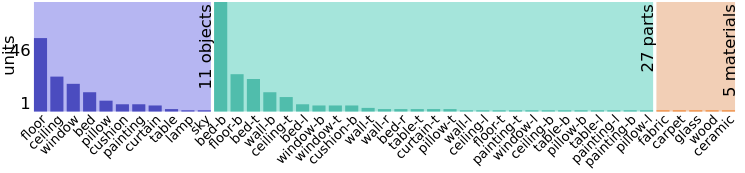
\includegraphics[scale=0.3]{images/sg_layer6.png}
    \end{subfigure} &
    \begin{subfigure}[h!]{0.5\textwidth}
        \caption{Unit 511: bed 0.56 IoU}
        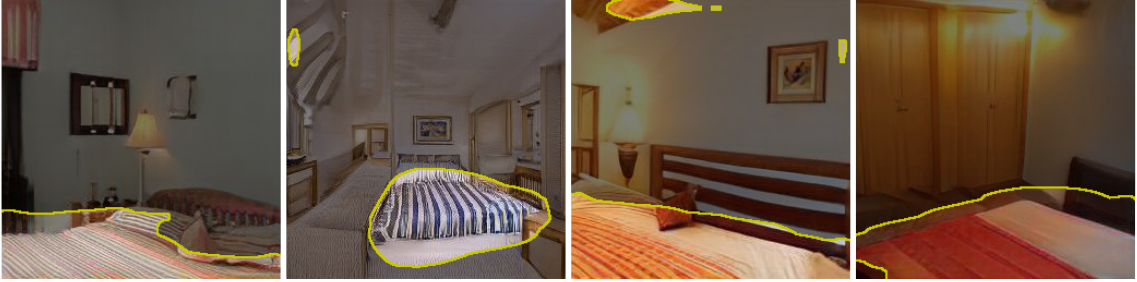
\includegraphics[scale=0.2]{images/sg_layer6_u511_bed_iou0.56.png}
    \end{subfigure} \\
    \begin{subfigure}[h!]{0.6\textwidth}
        \caption{Layer 9 interpretable units (128/256)}
        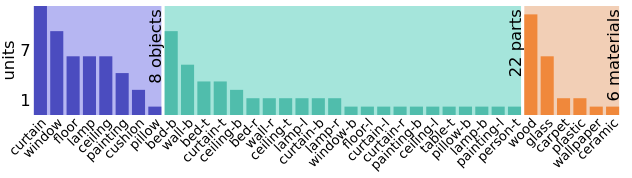
\includegraphics[scale=0.3]{images/sg_layer9.png}
    \end{subfigure} &
    \begin{subfigure}[h!]{0.5\textwidth}
        \caption{Unit 112: floor 0.37 IoU}
        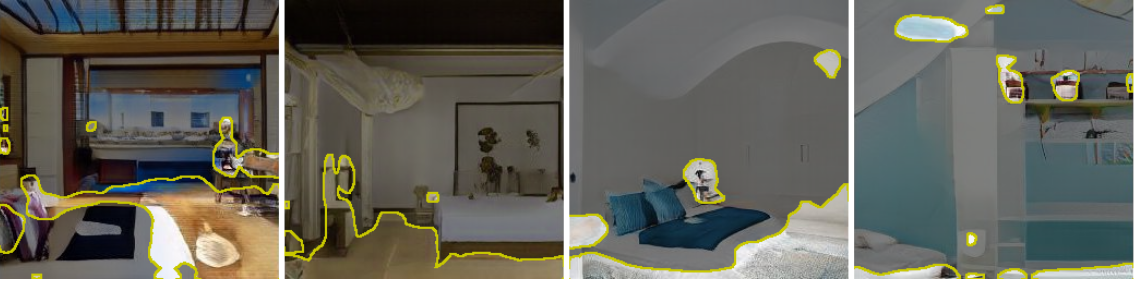
\includegraphics[scale=0.2]{images/sg_layer9_u112_flooriou_0.37.png}
    \end{subfigure} \\
    \begin{subfigure}[h!]{0.6\textwidth}
        \caption{Layer 11 interpretable units (39/128)}
        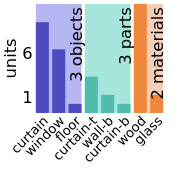
\includegraphics[scale=0.4]{images/sg_layer11.png}
    \end{subfigure} & 
    \begin{subfigure}[h!]{0.5\textwidth}
        \caption{unit 102 wood 0.32 IoU}
        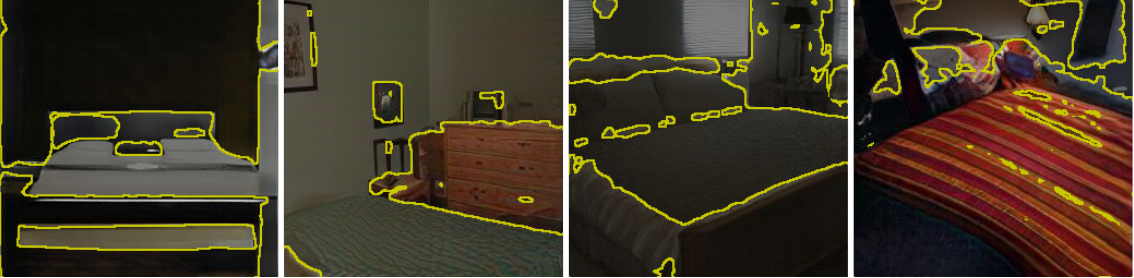
\includegraphics[scale=0.2]{images/sg_layer11_unit102_wood_0.32.png}
    \end{subfigure} \\
    \begin{subfigure}[h!]{0.6\textwidth}
        \caption{Layer 13 interpretable units (22/64)}
        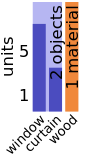
\includegraphics[scale=0.4]{images/sg_layer13.png}
    \end{subfigure} & 
    \begin{subfigure}[h!]{0.5\textwidth}
        \caption{unit 44 wood 0.24 IoU}
        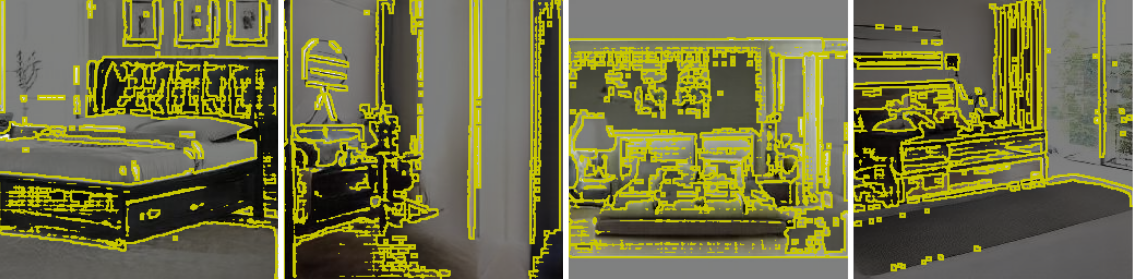
\includegraphics[scale=0.2]{images/sg_layer13_unit44_wood_0.24.png}
    \end{subfigure} \\
\end{tabular}
\end{figure}


For comparison, the highest IoU of any unit observed in the Progressive GAN we dissected was 0.32, and there are a significant number of units above that for styleGAN. We thought after seeing this that interventions would be really effective on these units, but we thought wrong. Also, we forgot to make the noise injections deterministic, so there were slight variations in the output image each time we reloaded it, and thus each time we carried out an intervention. In an ideal case for observing the effects of the interventions, this would be turned off so that you could see the full effect of the intervention, but we're not doing anything rigorous here and it looked kind of neat as we could see the variation that the noise injections introduced as we reloaded the images. 

It also had the unintended side effect of exposing us to a really interesting phenomenon. As we increased the number of units ablated or inserted, regardless of what type of unit we intervened with or whether we were inserting or ablating units, the noise variation seemed to increase the more units we intervened with. In fact, that's all that we really noticed, we couldn't remove or add objects to the image at all really. No matter how many units we shut off, the network was resilient to the change, and all we ended up doing was increasing the noisy-ness of the output. Eventually the image did end up looking pretty wonky, but that was only after shutting off most of the layer, and we didn't really achieve the removal of any objects, just distortions. Part of this, we think, is because the latent vector is embedded throughout the network, so the image itself is represented across many layers, and the object representations were too distributed over several layers to be removed by interventions. In a sense, the latent embedding had already dictated the objects that appear in the image, and we could only slightly alter their "pose" or positions. 
The network wasn't completely resilient, though. We noticed at the later layers where the finer details like textures are being filled in that each unit plays a crucial role to the output image being "filled in", and shutting off even a few units was enough to completely distort the texture (not the objects) of the output.

\begin{figure}[h!]
\caption{Noise increase with ablation in Style GAN}
    \centering
    \begin{subfigure}[h!]{0.35\textwidth}
        \caption{Layer 11 unaltered image}
        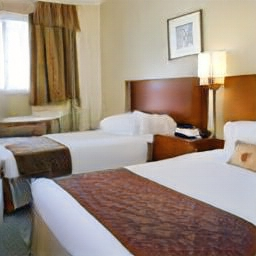
\includegraphics[scale=0.3]{images/sg_layer11_no_ablate.jpg}
    \end{subfigure}
    \begin{subfigure}[h!]{0.35\textwidth}
        \caption{Layer 11 5 units ablated}
        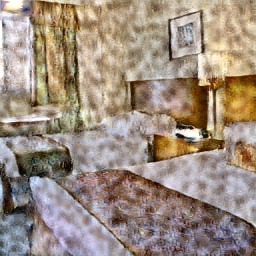
\includegraphics[scale=0.3]{images/sg_layer11_5_units_ablate.jpeg}
    \end{subfigure}
\end{figure}

And with regard to the increasing "noisy" variations as we add more and more interventions to a layer, we aren't really familiar enough with StyleGAN's architecture to really have a good guess as to why it happens, but it is an interesting phenomenon. 

\begin{figure}[H]
    \caption{The top row shows slight variations with no intervention due to noise injection, the bottom row shows the increased sensitivity to noisy variation with a significant number of units on layer 6 shut off (its perhaps more obvious in GIF format)}
\hspace{-2.5em}\begin{tabular}{c c c c}
    \begin{subfigure}[h!]{0.25\textwidth}
        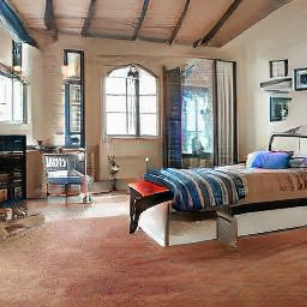
\includegraphics[scale=0.35]{images/n1.png}
    \end{subfigure} & 
     \begin{subfigure}[h!]{0.25\textwidth}
        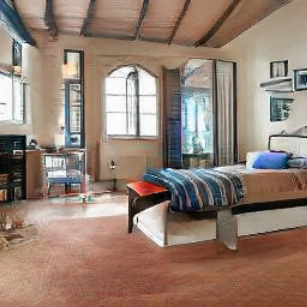
\includegraphics[scale=0.35]{images/n2.png}
    \end{subfigure} &
     \begin{subfigure}[h!]{0.25\textwidth}
        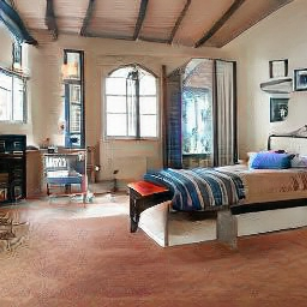
\includegraphics[scale=0.35]{images/n3.png}
    \end{subfigure} &
     \begin{subfigure}[h!]{0.25\textwidth}
        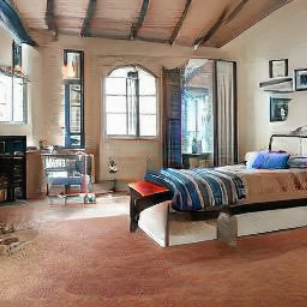
\includegraphics[scale=0.35]{images/n4.png}
    \end{subfigure}\\
     \begin{subfigure}[h!]{0.25\textwidth}
        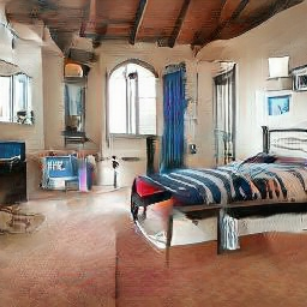
\includegraphics[scale=0.35]{images/a1.png}
    \end{subfigure} &
     \begin{subfigure}[h!]{0.25\textwidth}
        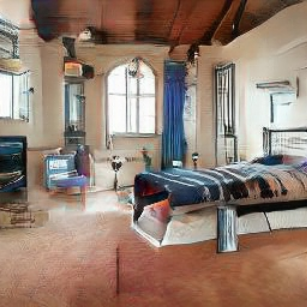
\includegraphics[scale=0.35]{images/a2.png}
    \end{subfigure} &
     \begin{subfigure}[h!]{0.25\textwidth}
        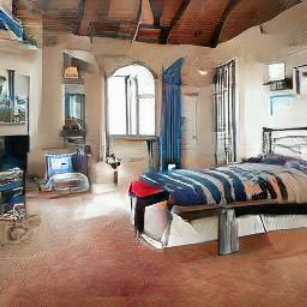
\includegraphics[scale=0.35]{images/a3.png}
    \end{subfigure} &
     \begin{subfigure}[h!]{0.25\textwidth}
        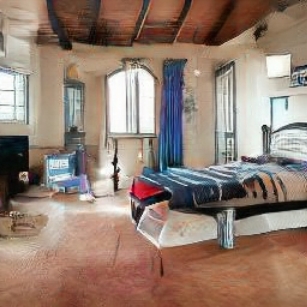
\includegraphics[scale=0.35]{images/a4.png}
    \end{subfigure} \\
    \end{tabular}
\end{figure}

Also, if you look closely, you'll notice that it's not entirely the case that we cannot remove objects from the image, as there is one object that is constantly missing. Which brings us to our last, and also most interesting observation...
\section{Unit 59}
We noticed that after ablating enough units, we were able to remove single, distinct pillows off of beds pretty consistently. We decided to examine this further, and found an image with such a pillow to determine how many units we'd have to shut off to make the pillow disappear, and what we noticed was a rather stark transition:

\begin{figure}[H]
    \centering
    \begin{subfigure}{.3\textwidth}
        \caption{no pillow units ablated}
        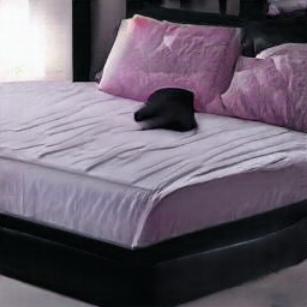
\includegraphics[scale=0.28]{images/black_pillow_no_ablate.png}
    \end{subfigure}
    \begin{subfigure}{.3\textwidth}
        \caption{top 28 pillow units ablated}
        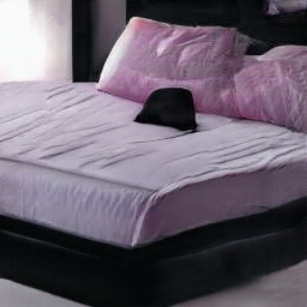
\includegraphics[scale=0.28]{images/black_pillow_top28.png}
    \end{subfigure}
    \begin{subfigure}{.3\textwidth}
        \caption{top 29}
        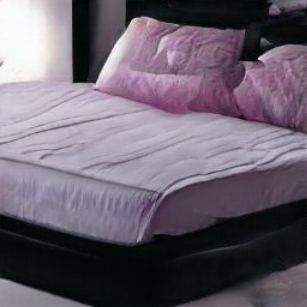
\includegraphics[scale=0.28]{images/black_pillow_top29.png}
    \end{subfigure}
\end{figure}

Could it be that 29 is the magical number of pillow units that needed to be ablated before we could remove the pillow? We decided to look into it, and found the specific unit that we ablated to send it over the threshold, unit 59, layer 6. We then reactivated all of the other units and found that unit 59 was not the straw that broke the camels back, but rather unit 59 was the sole causal factor of the pillow's disappearance. We then looked at other bedroom pictures with pillows (not the big pillows that are on every bed, but the distinct small "cushions" is what the segmenter calls them) and found that whichever picture we found with a small cushion, unit 59 would erase it. Unit 59 was in fact the one-hot encoding of such cushions in the image, and we could remove any cushion by ablating it, and (often, not always, so not technically one-hot) add cushions by inserting unit 59. 

\section{Conclusion}
Our results for pix2pix were somewhat lackluster, but we don't think that represents a dead end. There are many more avenues (and layers, we only did three) with which the model could be examined and might provide some interesting insights. StyleGAN on the other hand gave us some exciting results in the end, which we think invite further study. In particular, through what effect do interventions drive the amplification of noise, and might there be more ways of identifying units with extreme causal effect like that of unit 59? 

While we maybe had higher hopes for our pix2pix experiment, we think that the experience gained through the process was worth it. And while we thought we'd be able to exercise more control over the styleGAN output, we're pretty intrigued by the findings that we got. This has ultimately served as a learning experience for all of us, and we're glad to have had it.

\bibliography{papers}



\end{document}